% begin Chapter ProposedSolution

\chapter {Gaman: A solution prototype}
\label{chapter-SolutionPrototype}

\paragraph {} So far we have seen how the problem of the public transport system is structured and how it affects the stakeholders. We also saw how the nature of the problem demands a Decision Support System-like solution. This Chapter attempts to propose a DSS that deals with the public transportation problem. The architecture of the proposed system will be provided along with the proposed system features. The Chapter will end with a few UI screenshots of the prototype that was developed to test the usability and effectiveness of the functionality with the users.

\section{System Architecture}

\paragraph{ } The proposed system is designed as a web application following the client-server model. This design is the most conducive to the problem as it enables access to all stakeholders concerned in a distributed fashion. Therefore, commuters can access the system on-demand while allowing the schedulers access to the system and the data in real-time.

The prototype system used the three-tier architecture in the application. This architecture was chosen because it allowed the development of the prototype to be faster and more easily adaptable to possible requirements changes. The technologies used for the prototype are listed below,

\begin {itemize}
\item Programming Language: PHP
\item Database: MySQL
\item Versioning System: GitHub
\item UI Framework: Twitter Bootstrap
\item Theme: Flatly theme by Bootswatch (Source: http://bootswatch.com/2/flatly/)
\end {itemize}

The software architecture of the system is depicted in Figure~\ref{image-proposedSystemArchitecture}. (subsystems are outlined in red dashes)

\begin {figure} [h!]
\centering
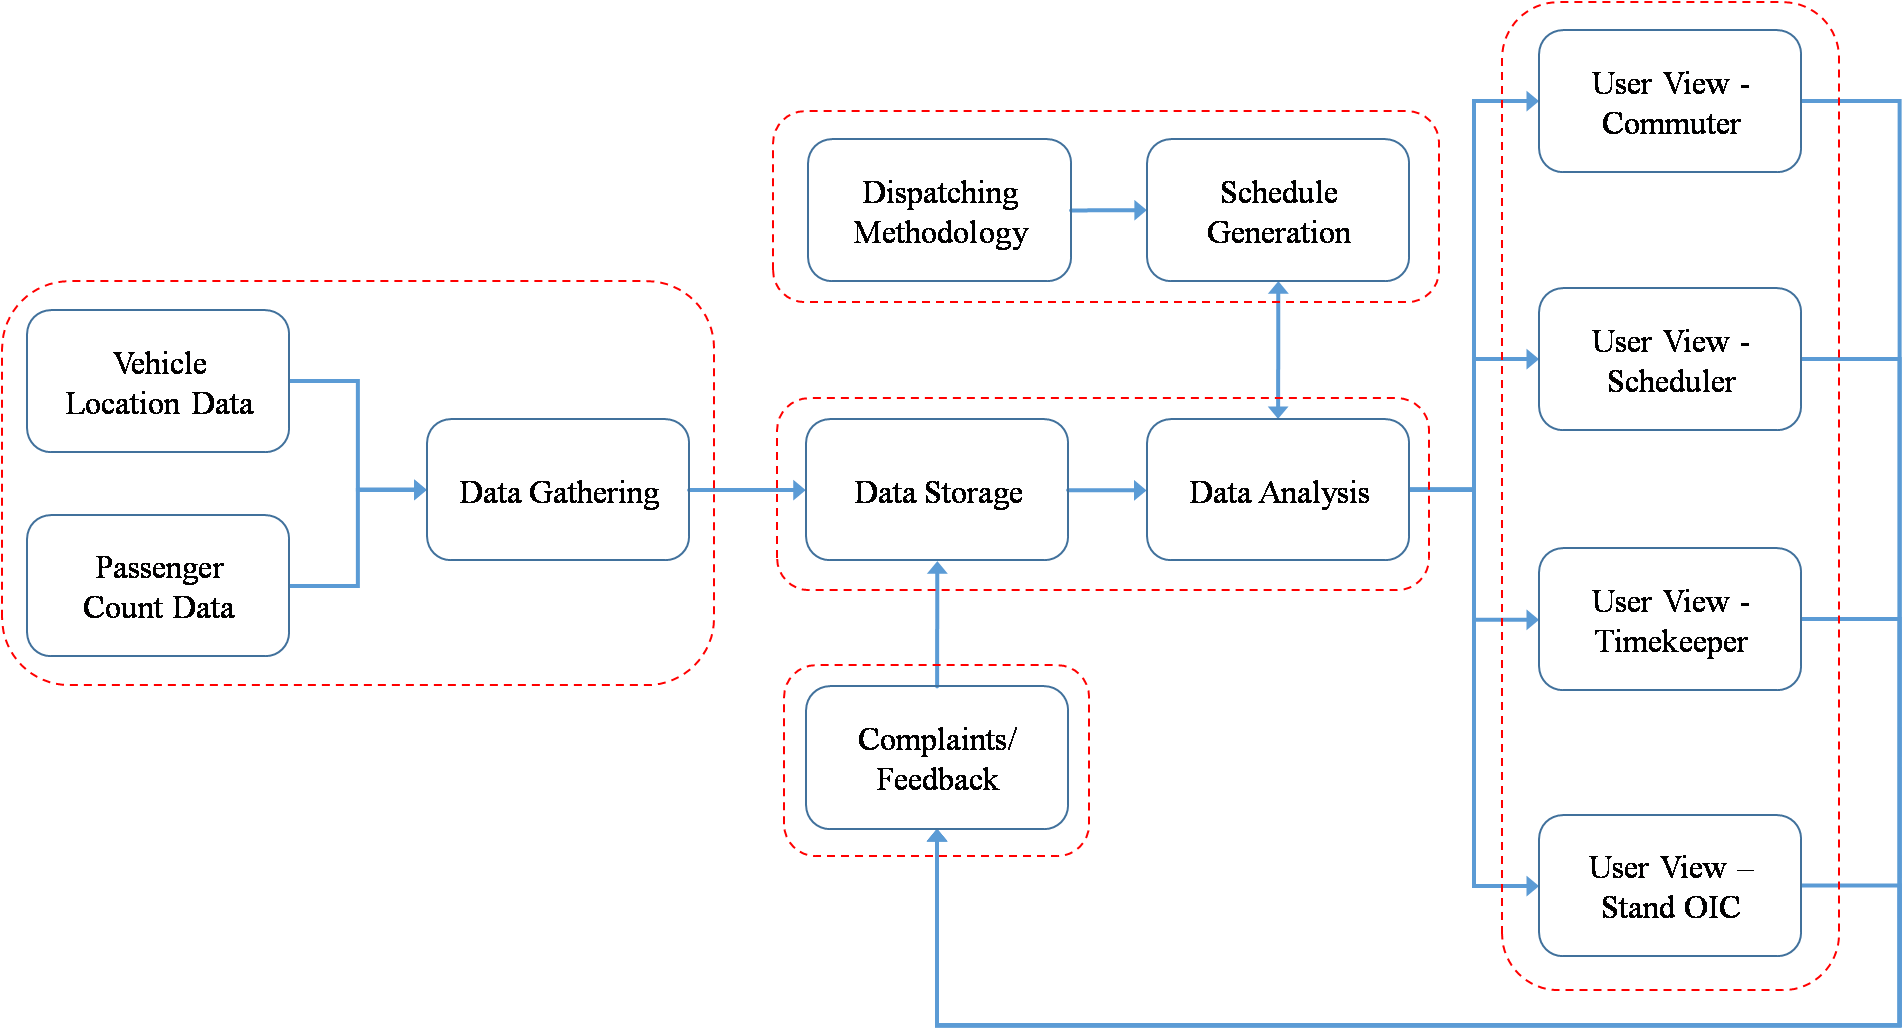
\includegraphics [scale=0.45] {proposedSystemArchitecture}
\caption [Proposed System Architecture] {Proposed System Architecture}
\label {image-proposedSystemArchitecture}
\end {figure}

The prototype that was created only included a subset of this whole architecture due to time and resource constraints. Also of note is the fact that the Data Gathering subsystem involves the data gathering infrastructure and is beyond the scope of this research project. However, it is an imperative aspect of the whole system.

\subsection{System Entities \& their Relationships}

\paragraph{} The Proposed System works with 4 main entities at it's core. They are,

\begin {itemize}
\item \textbf{Bus Routes} - Bus Routes refer to the routes that the buses provide the service on. They consist of a Beginning Bus Stop, an Ending Bus Stop and Bus Stops in between. One Bus Route may have many Stops
\item \textbf{Bus Stops} - This refers to the place allocated for a Bus to stop and drop off and/or pick up passengers. This is also known as the Bus Stand
\item \textbf{Buses} - This refers to the individual Buses that operate and provide the service to the commuters. One Bus is assigned to only one Bus Route. One Bus may have many Bus Personnel attached to it.
\item \textbf{Bus Personnel} - This refers to the people involved with the operation of the buses. This includes the Bus Driver, the Bus Conductor and the Bus Owner. In certain instances, these roles overlap. Accordingly, there may be situations where a Bus Driver is also an Owner or a Bus Conductor who is also an Owner. Each Bus Person (singular of Personnel) is assigned to only one Bus.
\end {itemize}

\paragraph{} Apart from these 4 core entities, the \textbf{Complaints} and the \textbf{General Feedback} entities are present. They exist to provide much needed feedback to the schedulers so that service quality can be maintained. These entities provide the basis for the Feedback step in the timetabling process of the schedulers (For more information regarding this process, see Figure~\ref{image-timetablingProcessSteps}).

Additionally the \textbf{Survey}, \textbf{Trip} and \textbf{Stop Activity} entities exist to aid the Survey functionality of the schedulers. A brief intro into what these entities are is listed below,

\begin {itemize}
\item \textbf{Survey} - An investigation of the buses in a route in terms of the passenger loads on the buses plying on that route. These are called route surveys and the Schedulers say ascertain the passenger loads as input for the timetabling through this process. One Survey is conducted on only one route at a time.
\item \textbf{Trip} - A trip is one-way journey between the Beginning Stop and the Ending Stop of a Bus Route. A Survey has many Trips included. Within the Trip, there are many Stops, and consequently many Stop Activities.
\item \textbf{Stop Activity} - A Stop Activity is the record of the exchanges of passengers that occurs at a Bus Stop during a Trip. 4 main facts are recorded for a Stop Activity when the bus stops at a Bus Stop. The number of passengers who get off the bus, number of people that get on the bus, the time (timestamp) the bus came to a stop and the passengers started to get off the bus at the Bus Stop and finally the time (timestamp) the bus departed the Bus Stop.
\end {itemize}

The above mentioned entities allow the Schedulers to carry out a route survey and gather the necessary data for the timetabling process. The Route Surveys that the Schedulers perform are imperative in their timetable formulation as it acts as the data input for the process. The Schedulers mainly obtain the Passenger Load information which is directly related to the dispatching of buses on a route. Loiter time data is also used to identify errant bus operators as well as to continuously monitor the total travel time on a route.



\section{System Features}
\label{systemFeatures}

\paragraph{ } The list of system features and functionality is noted below. Please note, the features marked under \textit{Public} is available for the regular commuters to access while the functionality marked under \textit{Admin} is only available for the Schedulers and other administrative staff at the Transport Authority.

\begin{itemize}

\item Public Functions
\begin{itemize}
\item \textbf{Information Portal for Bus Routes, Stops, Buses and Bus Personnel} - This is, as its name suggests, the functionality of providing the data about the 4 main entities related to the transportation service in a smile easy-to-use, easy-to-read-and-understand interface. The information includes the basics from name of stop (for Bus Stops) and the Stops along a particular route (for Bus Routes) to more advanced things like the Personnel assigned to a particular Bus and the number of complaints received on a particular Bus.
\item \textbf{Information Portal for Bus Fares} - This would basically provide the details of the Bus fares in a given route.
\item \textbf{Bus Route Finder functionality} - When an origin and destination stop are given, the user is presented with a list of bus routes to take
\item \textbf{Submitting and reviewing submitted General Feedback} - Using this functionality, users can provide comments (good or bad) regarding the 4 main entities. This goes hand in hand with the Complaints and acts as a complimenting function to the Complaints.
\item \textbf{Submitting and reviewing submitted Complaints} - Users can submit their complaints to the authority and these will be investigated and action taken. The Complaints also acts as a notification for the Schedulers in their timetabling process. For instance when there are a lot of complaints on a particular route regarding overcrowded buses or consistently delayed buses, the Schedulers can reconsider the timetable for that route and improve it. Currently this connection between the Complaints and the Schedulers is not available and therefore the Schedulers have no idea which areas need improvement.
\end{itemize}

\item Admin Functions
\begin{itemize}
\item \textbf{Survey data storage, retrieval and visualization} - this is one of the main functionalities of the proposed system. it provides the knowledge base as well as the main input to the timetabling process of the Schedulers.
\item \textbf{Timetable Storage, Retrieval and Visualization} - Timetables are documents that the buses are dispatched according to. The tracking of buses according to their dispatch times is currently done manually. The times that the buses are dispatched are recorded on timetable and sent in to the regional offices. This functionality of the system attempts to digitize that by having a digital representation of the data so that it can be stored and retrieved later.
\item \textbf{Timetable Generation} - This functionality enables the schedulers to automatically generate timetables for a given route. As mentioned previously, this is currently done manually and the proposed system would incorporate a the feature of generating the timetable by calculating the average headways.
\item \textbf{Vehicle and Crew Scheduling} - This is the next step in the planning process. The Vehicle and Crew Scheduling functions are the rosters that the bus operators follow. This function enables the Schedulers to automatically generate these without having to do this step of the process manually.
\item \textbf{Complaint and General Feedback tracking Dashboard} - The Complaint and General Feedback functions serve as the indicator in this system. It tells the Schedulers which routes are doing well and which ones aren't, which buses are breaking the law and which bus personnel has a good record. It allows the authority to analyze the quality of the service and includes the commuters in the process of measuring service quality.
\end{itemize}

\end{itemize}



\section{URL of prototype system}

\paragraph{} The prototype system can be found at the following URL: \url{http://gaman.byethost4.com/}. The system's Admin Interface can be found at \url{http://gaman.byethost4.com/admin/}. The login credentials for both these interfaces are listed below.

\begin {itemize}

\item Public Area
\begin {itemize}
\item Username: \textbf{heisenberg}
\item Password: \textbf{123}
\end {itemize}

\item Admin area
\begin {itemize}
\item Username: \textbf{admin}
\item Password: \textbf{123}
\end {itemize}

\end {itemize}

The system is an active project on GitHub. The code repository can be found at, \url{https://github.com/afthaj/Gaman/}



\section{UI Screenshots}

\paragraph{} UI Screenshots of the prototype system are displayed below.


\begin {figure} [h!]
\centering
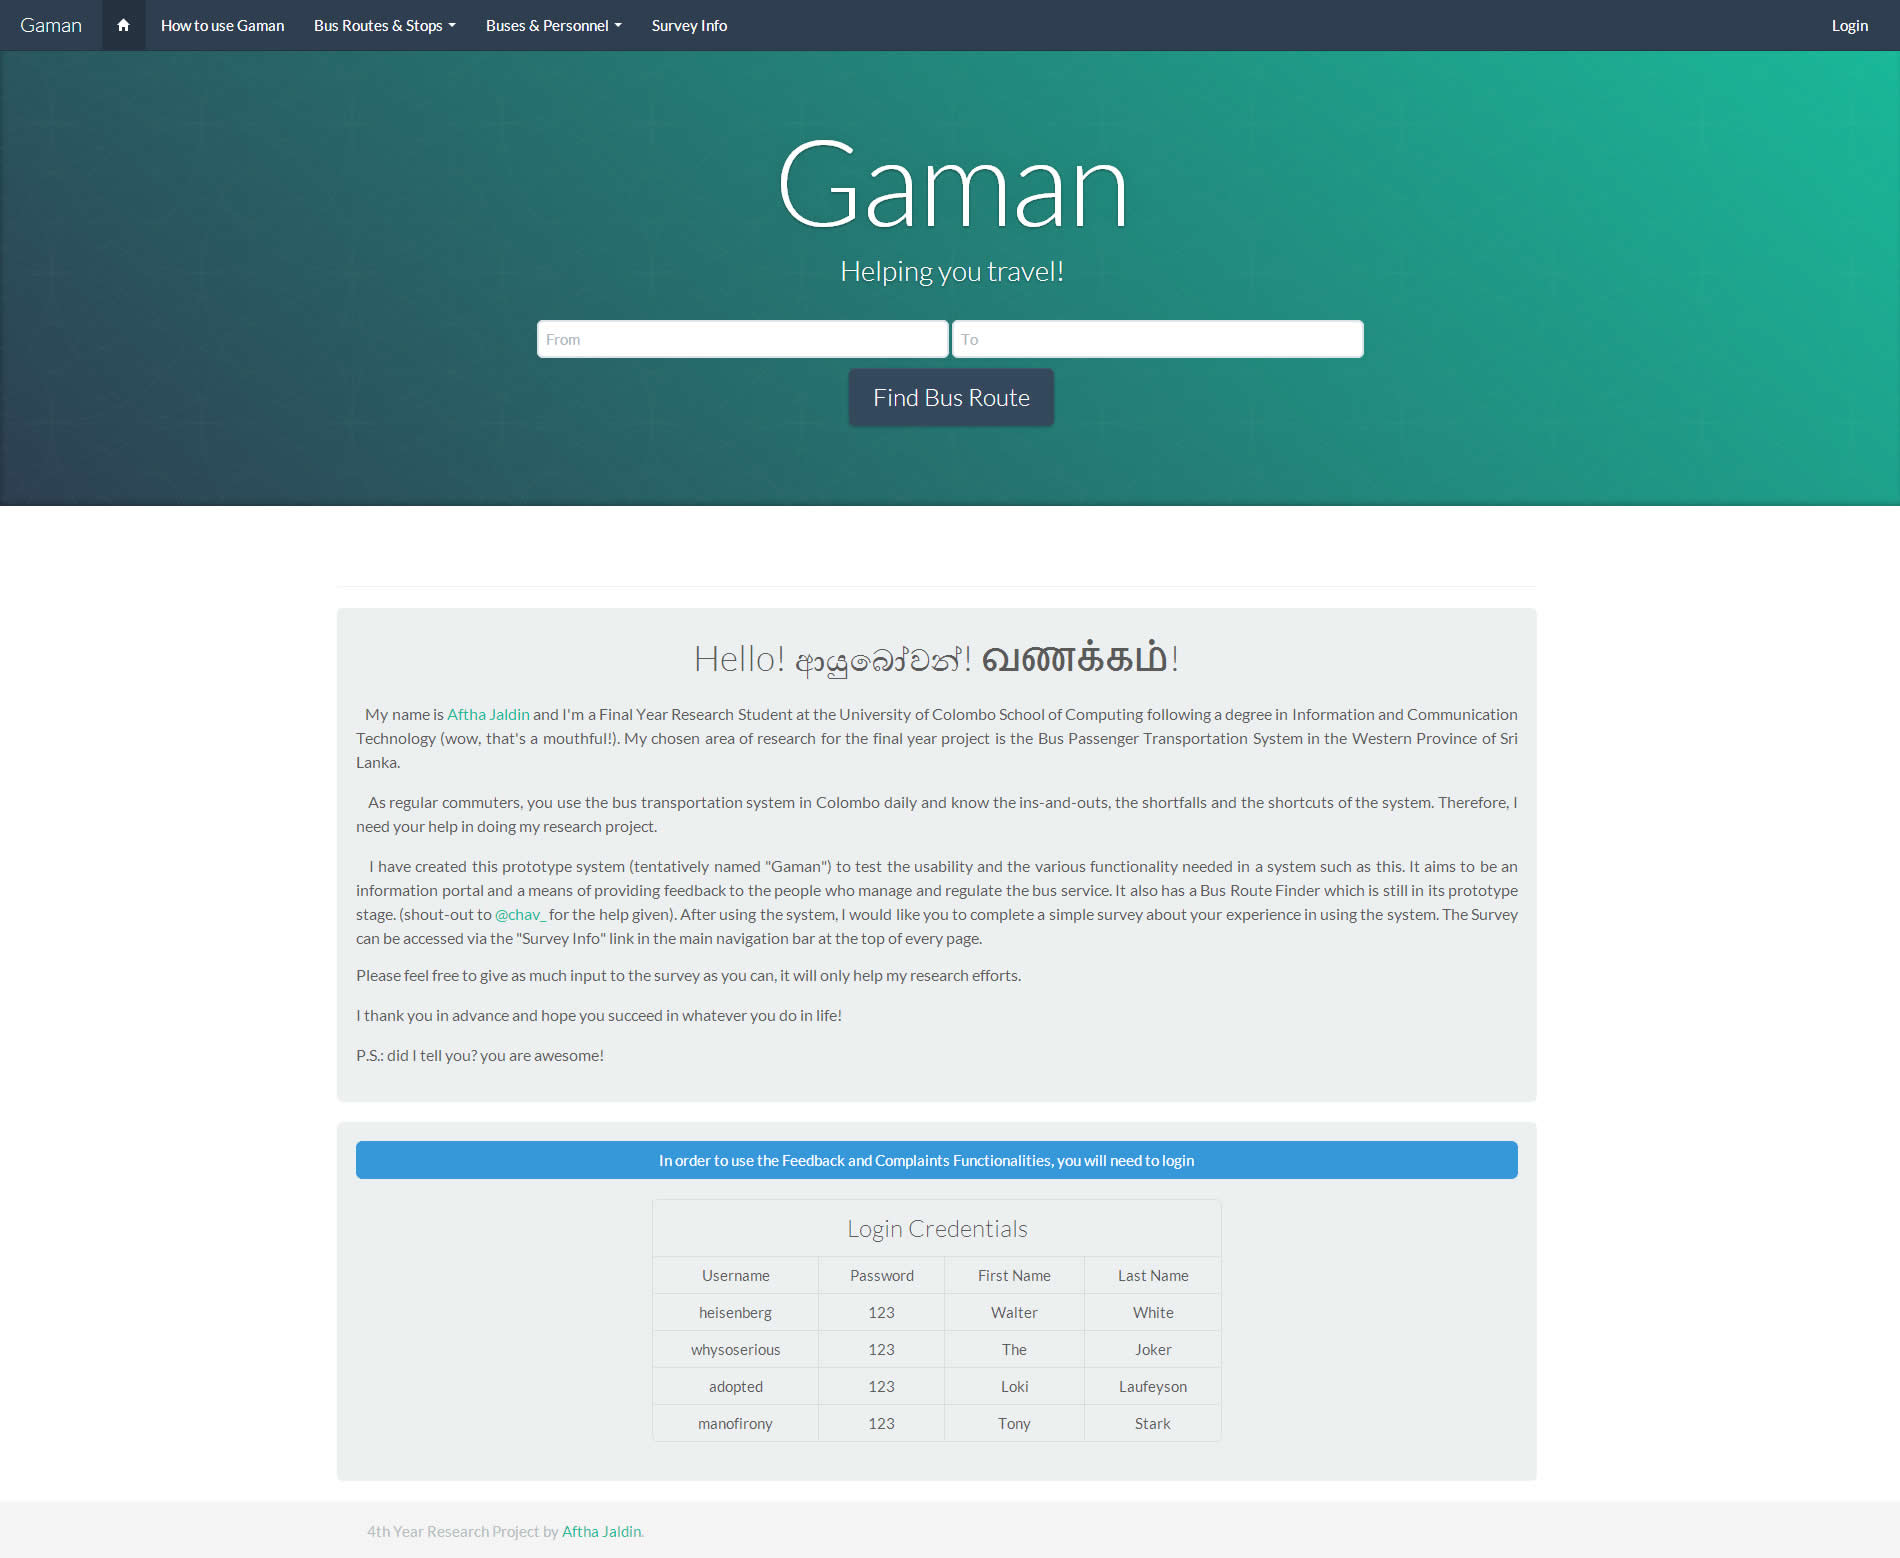
\includegraphics[scale=0.2]{homePage}
\caption [Screenshot - Home Page] {Screenshot - Home Page}
\label {image-homePage}
\end {figure}

\begin {figure} [h!]
\centering
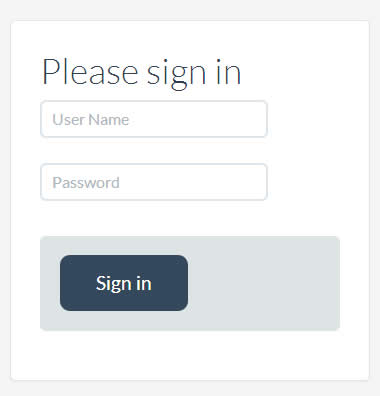
\includegraphics[scale=0.5]{loginPage}
\caption [Screenshot - Login Page] {Screenshot - Login Page}
\label {image-loginPage}
\end {figure}

\begin {figure} [h!]
\centering
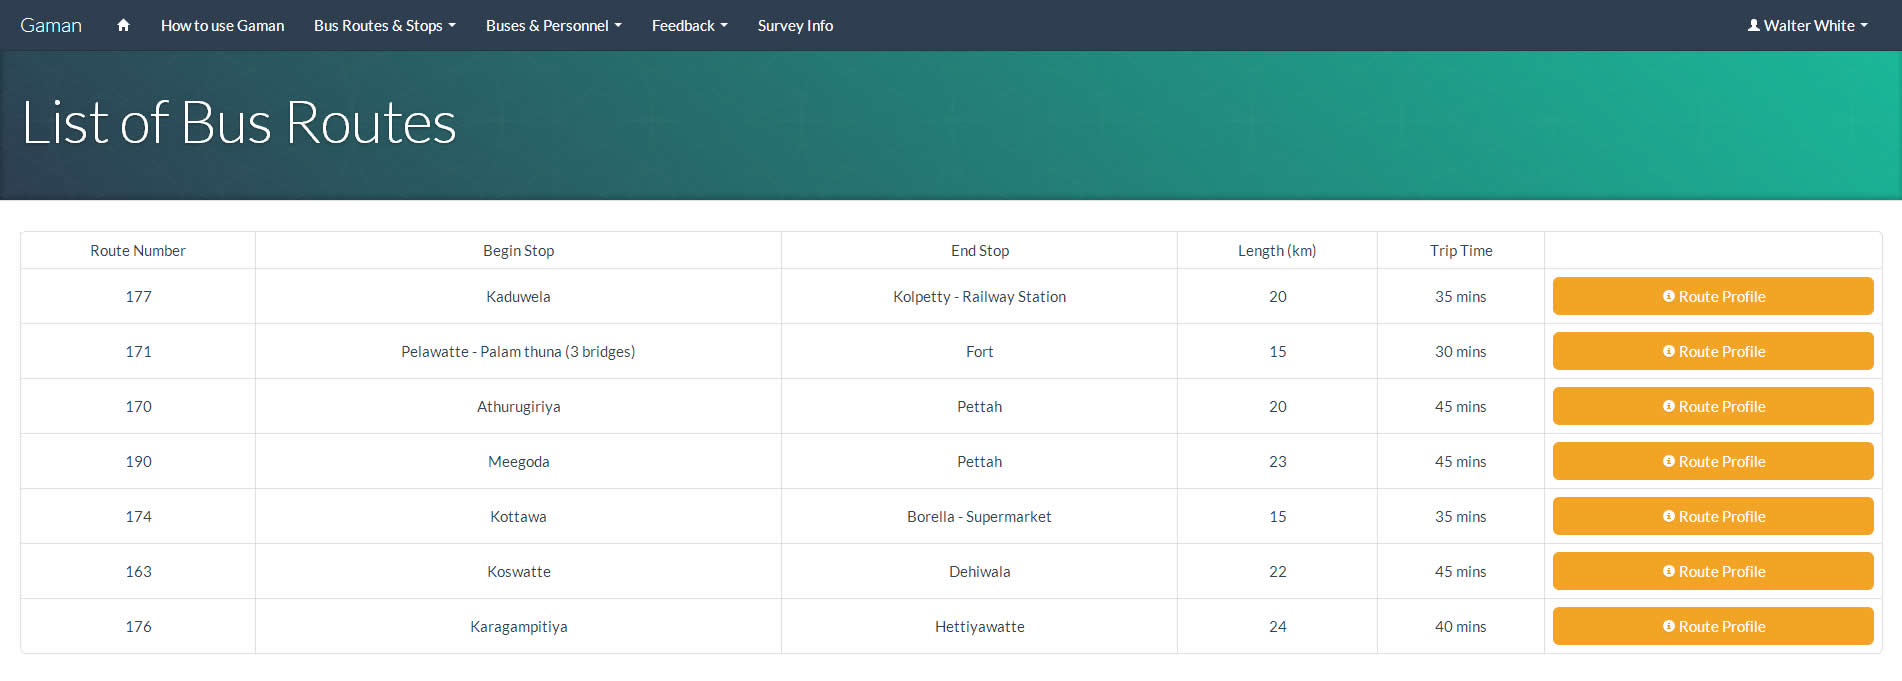
\includegraphics[scale=0.2]{listRoutes}
\caption [Screenshot - List of Routes] {Screenshot - List of Routes}
\label {image-listRoutes}
\end {figure}


\begin {figure} [h!]
\centering
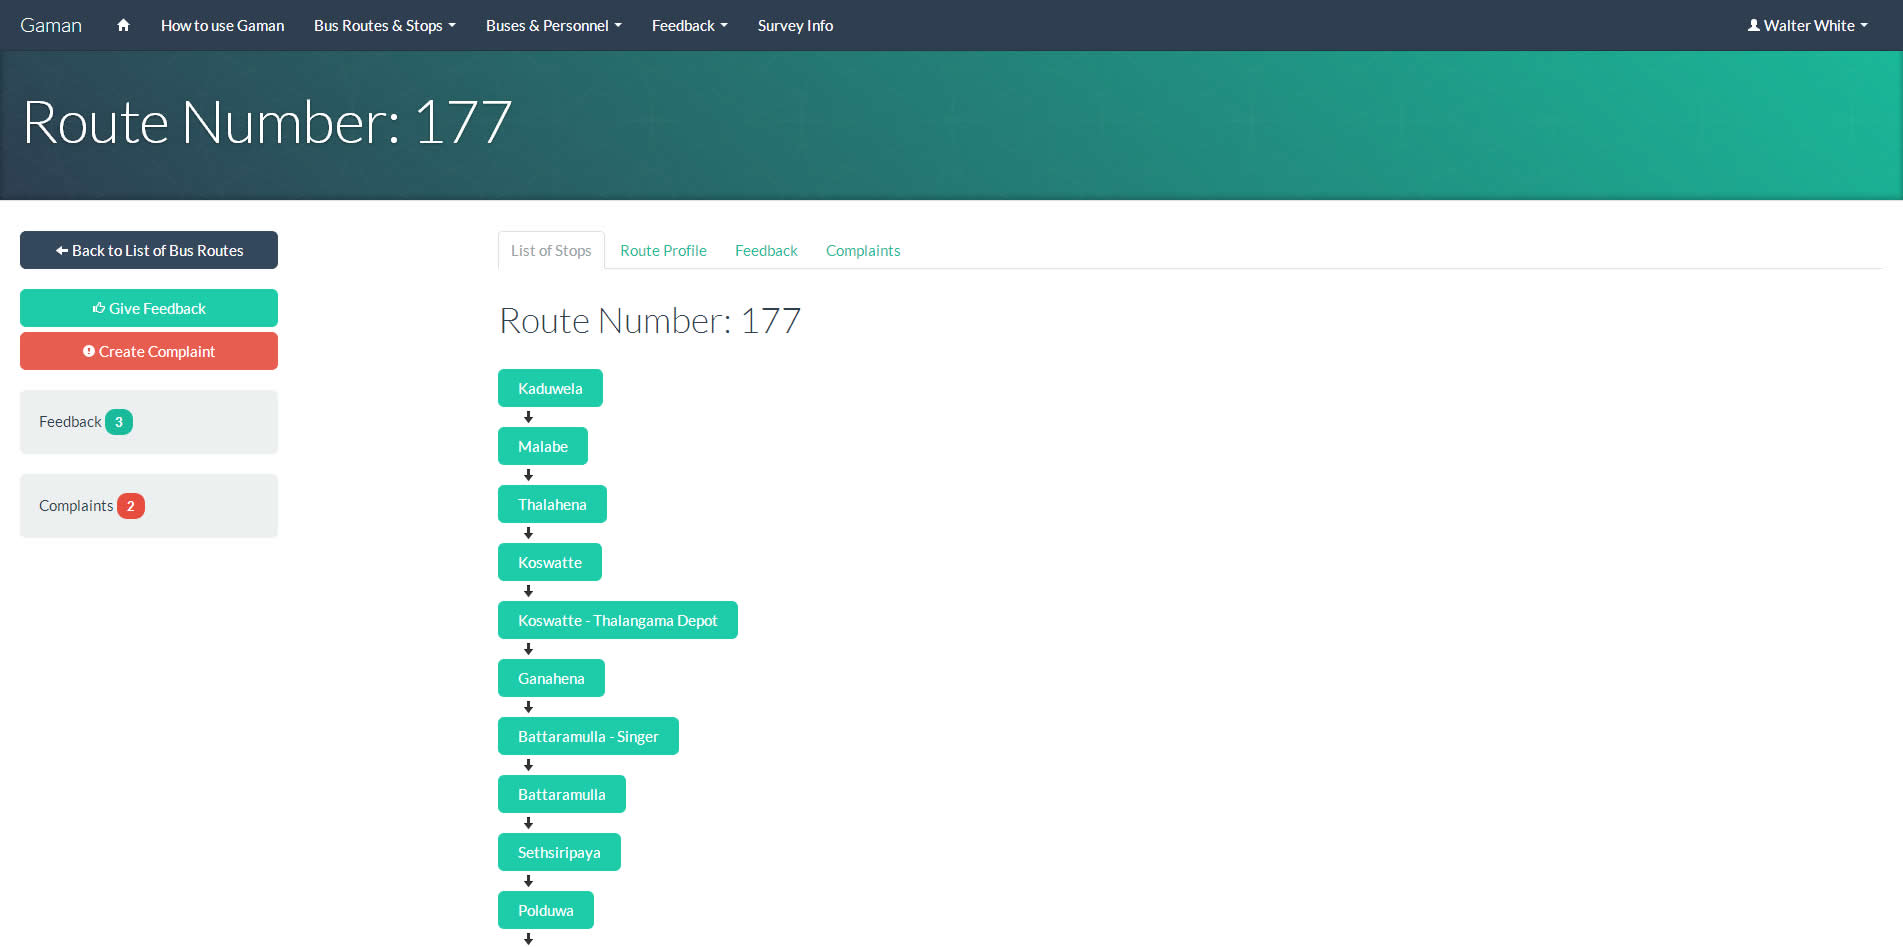
\includegraphics[scale=0.2]{viewRoute1}
\caption [Screenshot - View Route 1] {Screenshot - View Route 1}
\label {image-viewRoute1}
\end {figure}


\begin {figure} [h!]
\centering
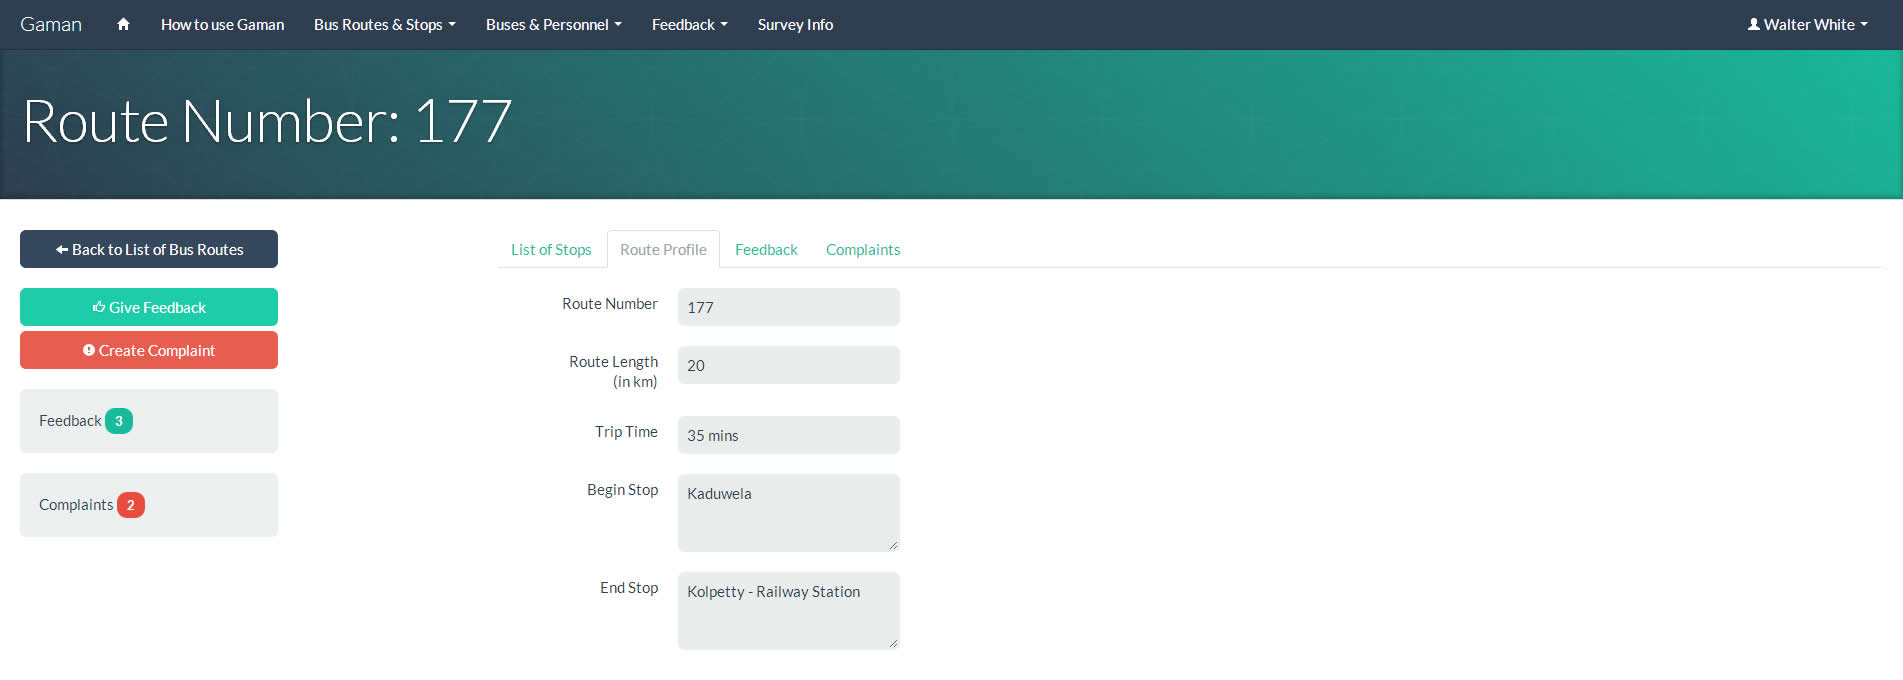
\includegraphics[scale=0.2]{viewRoute2}
\caption [Screenshot - View Route 2] {Screenshot - View Route 2}
\label {image-viewRoute2}
\end {figure}


\begin {figure} [h!]
\centering
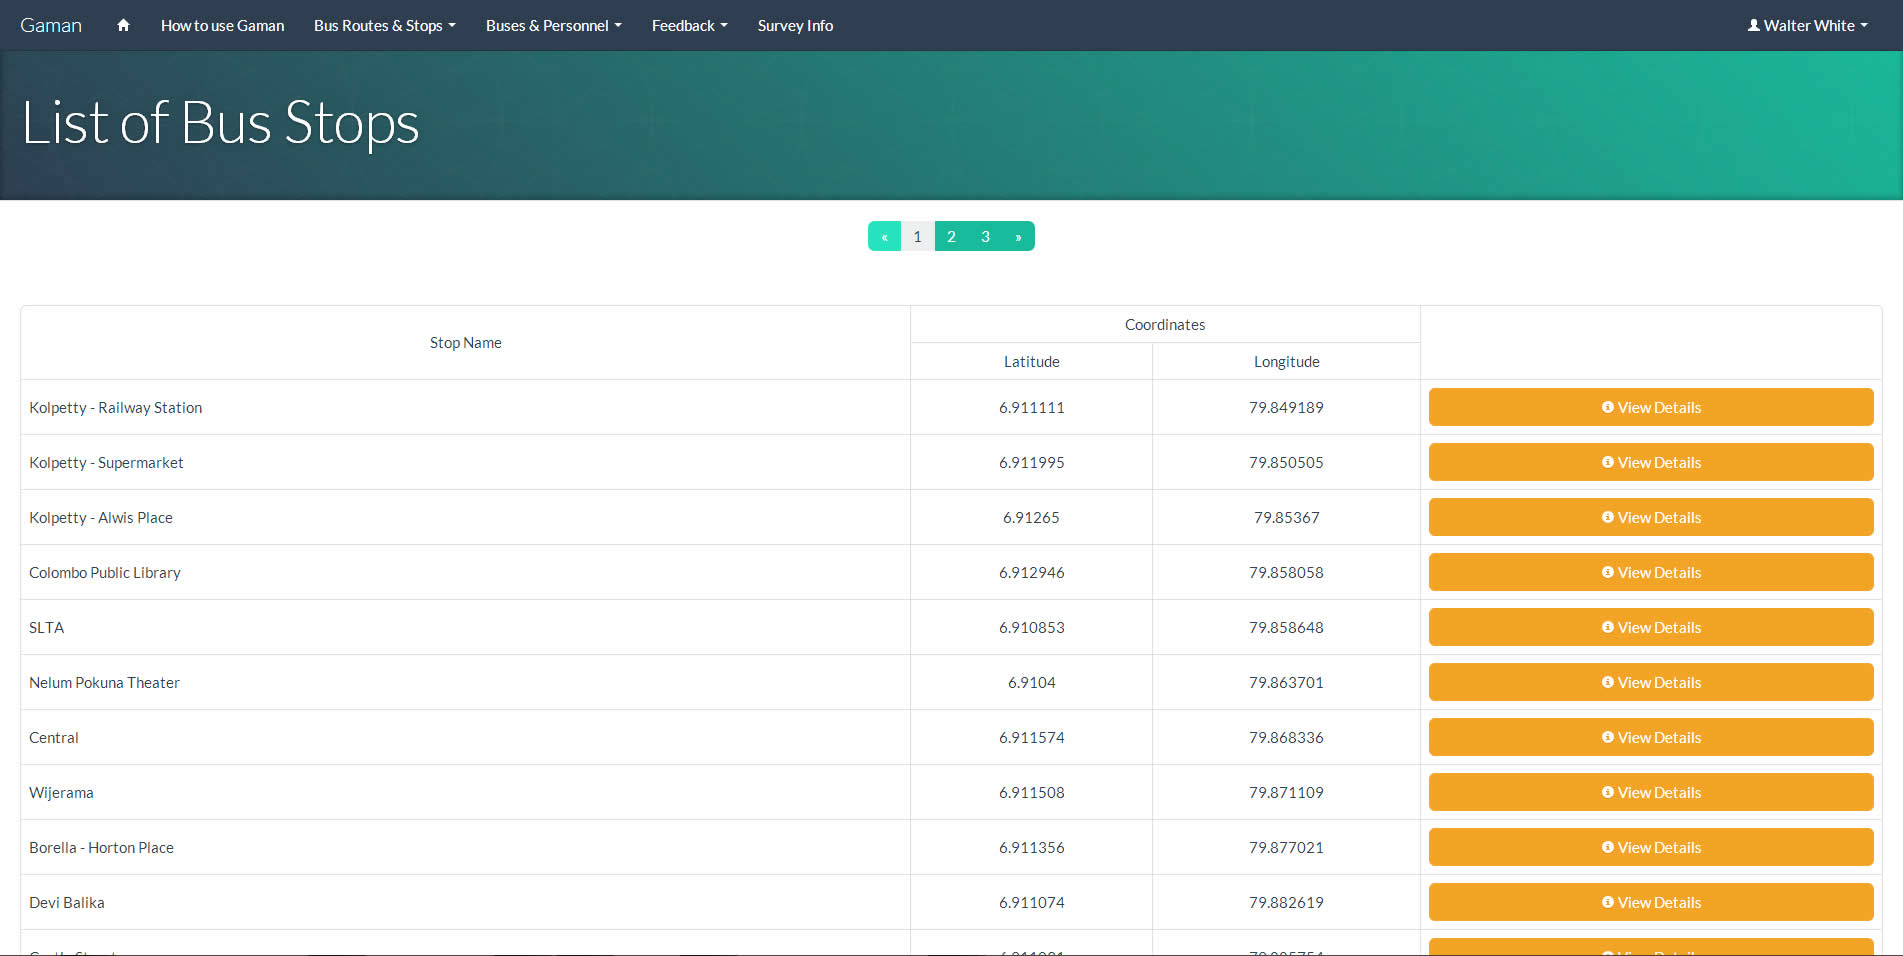
\includegraphics[scale=0.2]{listStops}
\caption [Screenshot - List of Stops] {Screenshot - List of Stops}
\label {image-listStops}
\end {figure}


\begin {figure} [h!]
\centering
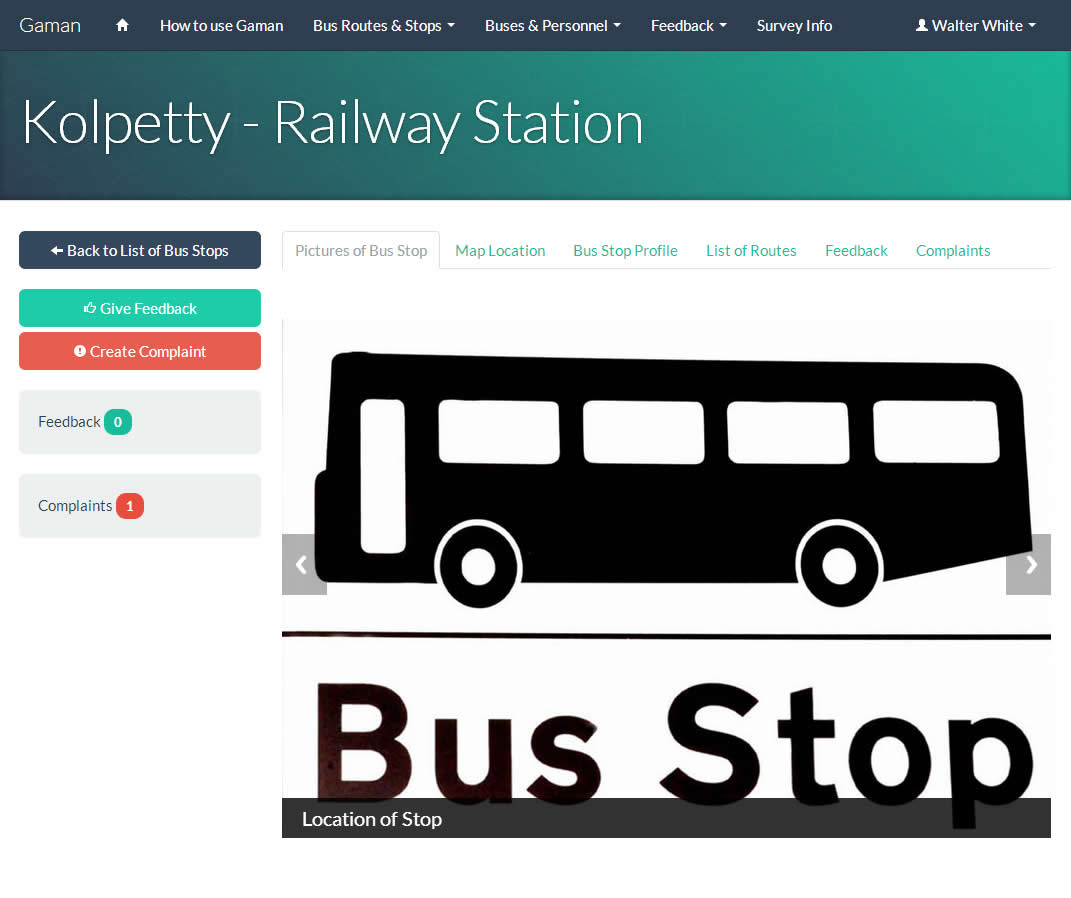
\includegraphics[scale=0.2]{viewStop1}
\caption [Screenshot - View Stop 1] {Screenshot - View Stop 1}
\label {image-viewStop1}
\end {figure}


\begin {figure} [h!]
\centering
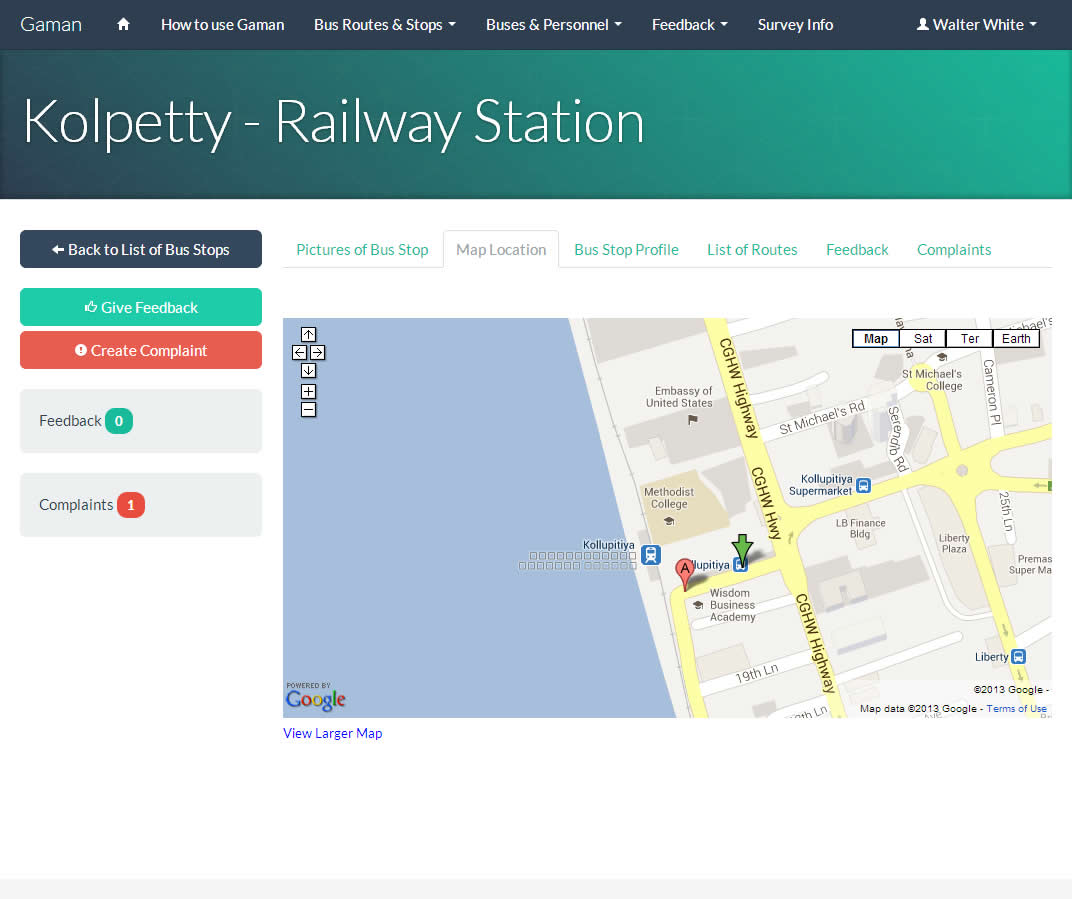
\includegraphics[scale=0.2]{viewStop2}
\caption [Screenshot - View Stop 2] {Screenshot - View Stop 2}
\label {image-viewStop2}
\end {figure}

\begin {figure} [h!]
\centering
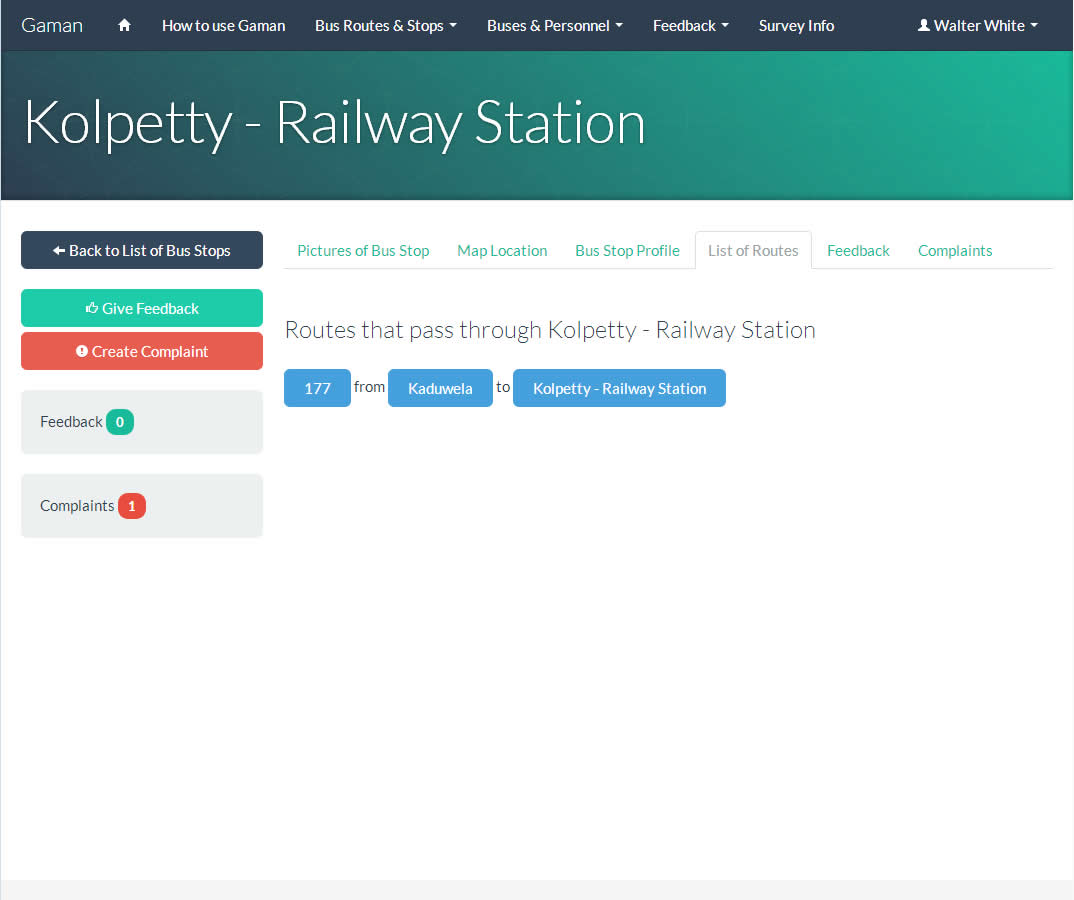
\includegraphics[scale=0.2]{viewStop3}
\caption [Screenshot - View Stop 3] {Screenshot - View Stop 3}
\label {image-viewStop3}
\end {figure}


\begin {figure} [h!]
\centering
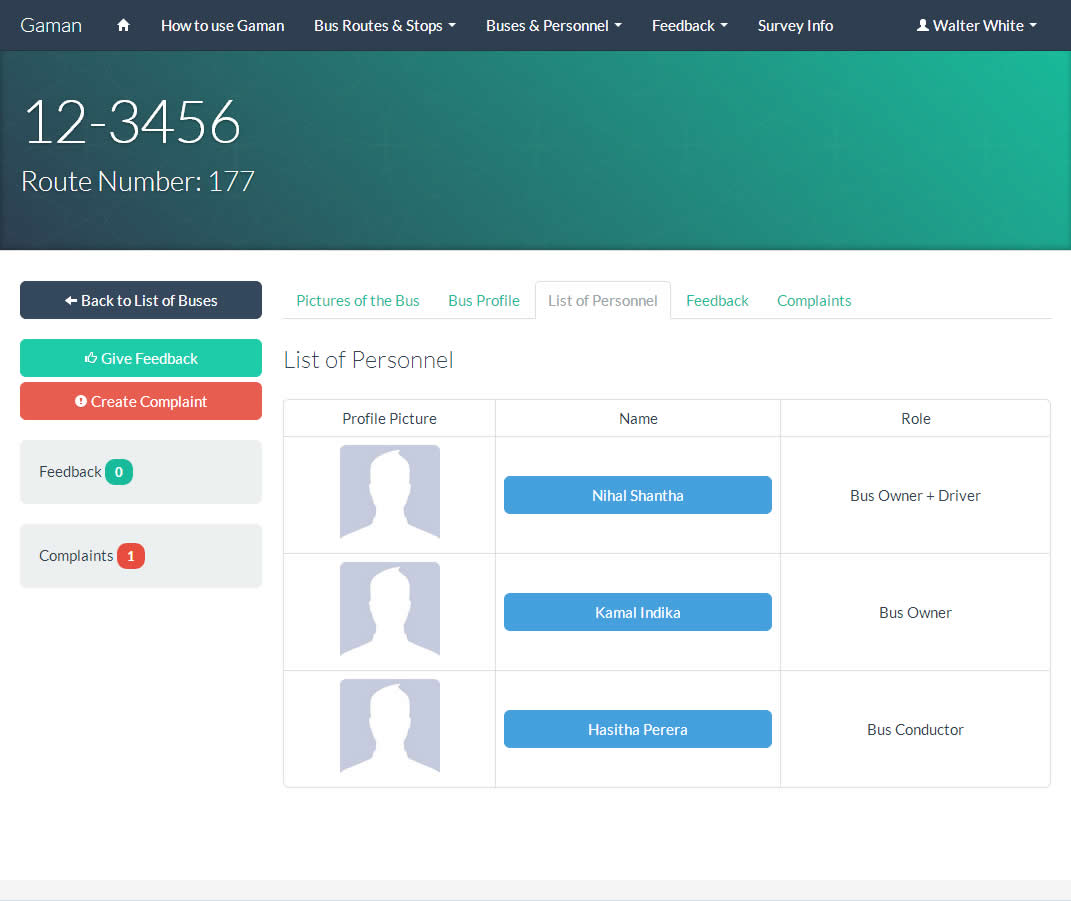
\includegraphics[scale=0.2]{viewBus1}
\caption [Screenshot - View Bus 1] {Screenshot - View Bus 1}
\label {image-viewBus1}
\end {figure}

\begin {figure} [h!]
\centering
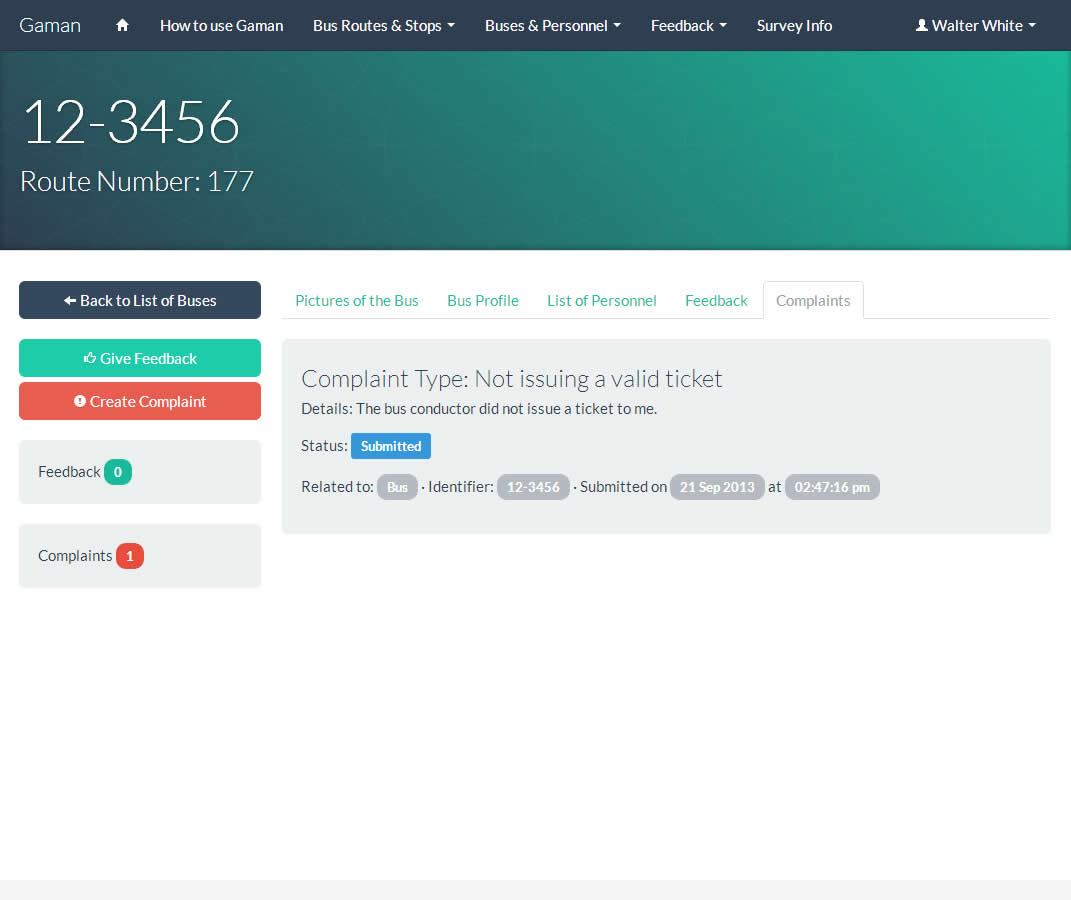
\includegraphics[scale=0.2]{viewBus2}
\caption [Screenshot - View Bus 2] {Screenshot - View Bus 2}
\label {image-viewBus2}
\end {figure}


\begin {figure} [h!]
\centering
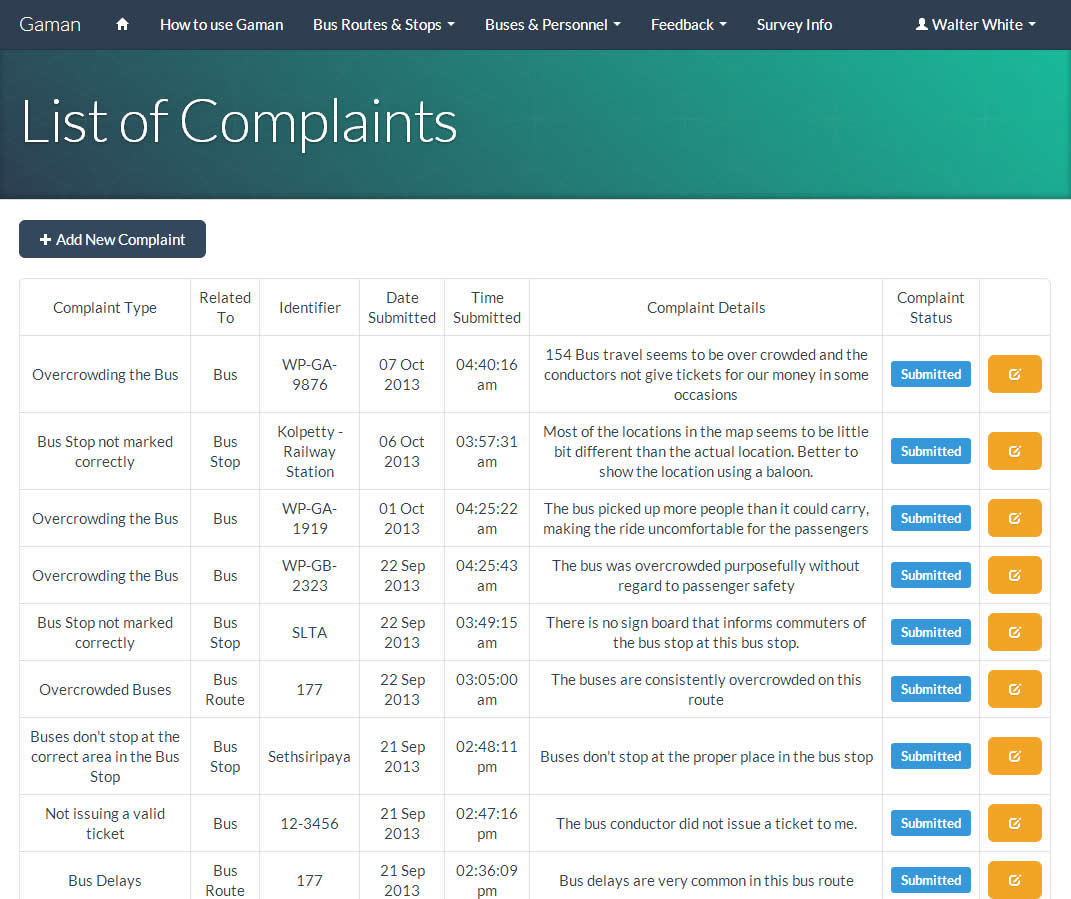
\includegraphics[scale=0.2]{listComplaints}
\caption [Screenshot - List of Complaints] {Screenshot - List of Complaints}
\label {image-listComplaints}
\end {figure}

\begin {figure} [h!]
\centering
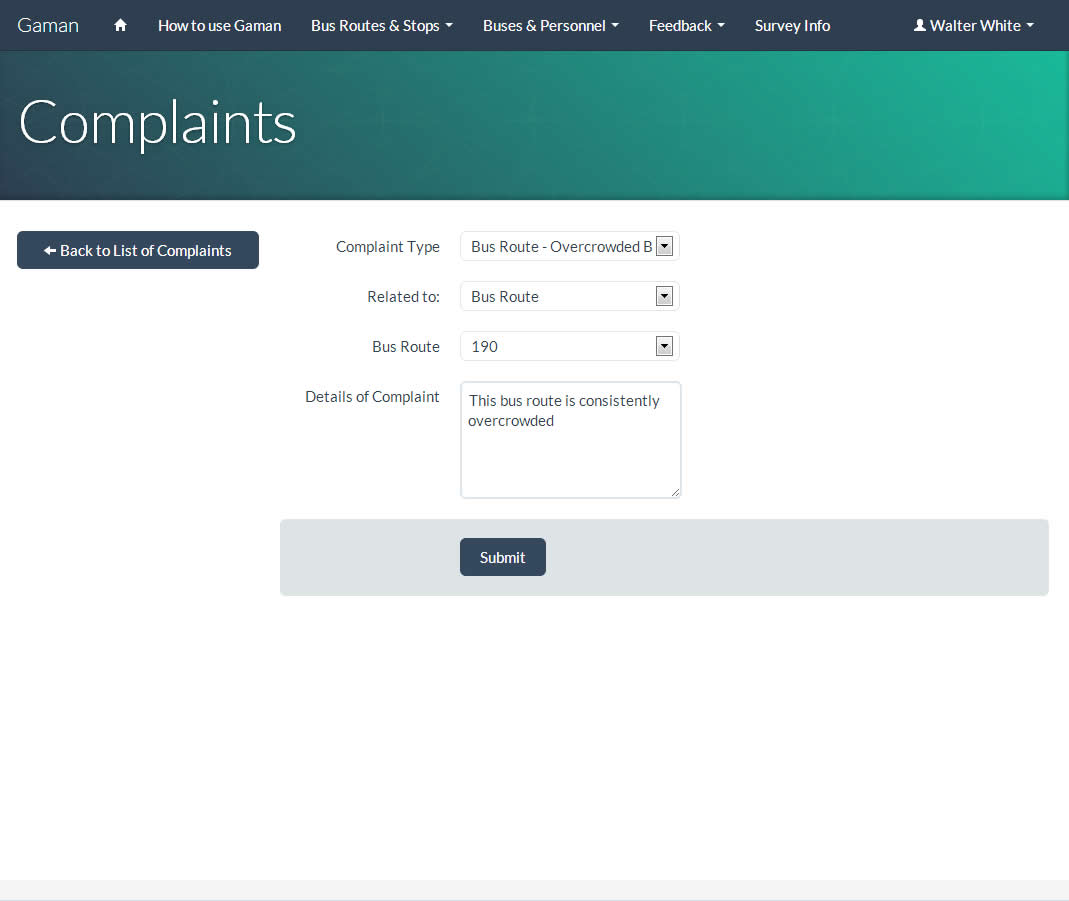
\includegraphics[scale=0.2]{addComplaint}
\caption [Screenshot - Add a Complaint] {Screenshot - Add a Complaint}
\label {image-addComplaint}
\end {figure}


\section{Testing the prototype}

\paragraph{} 